% !TEX root = knottedMain.tex
\documentclass[varwidth=\maxdimen]{standalone}

\usepackage{mathtools,amssymb,mathrsfs,dutchcal,upgreek,faktor,accents,etoolbox,multicol}
\usepackage[dvipsnames]{xcolor}
\definecolor{mygreen}{RGB}{	8,156,79 }
\usepackage{tikz,tikz-cd}


\usetikzlibrary{patterns,knots,arrows.meta,decorations.markings}
\tikzset{>={Straight Barb[scale=0.85]}}
\tikzcdset{
  cells={font=\everymath\expandafter{\the\everymath\displaystyle}},
  arrow style=tikz,
  diagrams={>={Straight Barb[scale=0.85]}},
  every label/.append style = {font = \small}
}

%%%%
% \tikzset{
% circle,fill,inner sep=0.8pt/.style={
%     circle,fill,inner sep=0.8pt
%     }
% }
\tikzset{
Decoration/.style={
    red,font=\footnotesize
    }
}
%%%%

\begin{document}
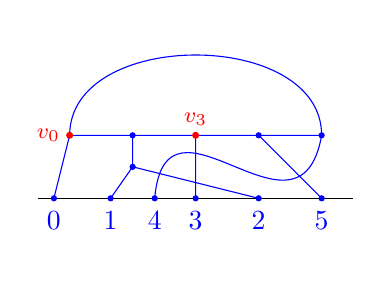
\begin{tikzpicture}[scale=0.8,even odd rule,baseline=0.5cm]
    \draw (-.5,0) -- (4.5,0);
    \draw[blue]
        (-0.25,0) node[circle,fill,inner sep=0.8pt,label=below:$0$]{} -- (0,1) node[red,circle,fill,inner sep=0.9pt]{} node[red,left]{\footnotesize$v_0$}-- (1,1) node[circle,fill,inner sep=0.8pt]{} -- (1,0.5) node[circle,fill,inner sep=0.8pt]{} -- (0.65,0) node[circle,fill,inner sep=0.8pt,label=below:$1$]{}
        (1,0.5)  --  (3,0) node[circle,fill,inner sep=0.8pt,label=below:$2$]{}
        (1,1) -- (2,1) node[red,circle,fill,inner sep=0.9pt]{} node[red,above]{\footnotesize$v_3$} -- (2,0) node[circle,fill,inner sep=0.8pt,label=below:$3$]{}
        (2,1) -- (3,1) node[circle,fill,inner sep=0.8pt]{} -- (4,0) node[circle,fill,inner sep=0.8pt,label=below:$5$]{}
        (3,1) -- (4,1) node[circle,fill,inner sep=0.8pt]{} to[out=-100,in=85,distance=2cm]  (1.35,0) node[circle,fill,inner sep=0.8pt,label=below:$4$]{}
        (4,1) to[out=90,in=90, distance=1.7cm]  (0,1) ;
\end{tikzpicture}$=$%
\begin{tabular}{c c}
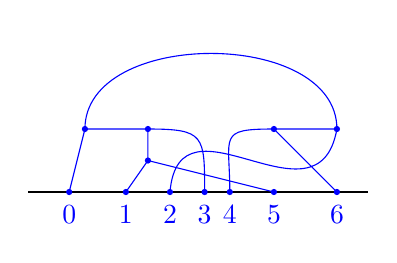
\begin{tikzpicture}[scale=0.8,even odd rule,baseline=0.5cm]
    % \draw[white,semithick] (5.6,1) -- (5.8,1) (5.6,0.9) -- (5.8,0.9);
    \draw (6.1,0) -- (11.5,0);
    \draw[blue]
        (6.75,0) node[circle,fill,inner sep=0.8pt,label=below:$0$]{} -- (7,1) node[circle,fill,inner sep=0.8pt]{} -- (8,1) node[circle,fill,inner sep=0.8pt]{}
        -- (8,0.5) node[circle,fill,inner sep=0.8pt]{} -- (7.65,0) node[circle,fill,inner sep=0.8pt,label=below:$1$]{}
        (8,0.5)  -- (10,0) node[circle,fill,inner sep=0.8pt,label=below:$5$]{}
        (8,1) to[out=0,in=90,distance=0.9cm] (8.9,0) node[circle,fill,inner sep=0.8pt,label=below:$3$]{}
        (9.3,0) node[circle,fill,inner sep=0.8pt,label=below:$4$]{} to[out=90,in=180,distance=0.9cm] (10,1) node[circle,fill,inner sep=0.8pt]{} -- (11,0) node[circle,fill,inner sep=0.8pt,label=below:$6$]{}
        (10,1) -- (11,1) node[circle,fill,inner sep=0.8pt]{} to[out=-100,in=85,distance=1.7cm] (8.35,0) node[circle,fill,inner sep=0.8pt,label=below:$2$]{}
        (11,1) to[out=90,in=90, distance=1.6cm]  (7,1) ;
\end{tikzpicture} &
$-$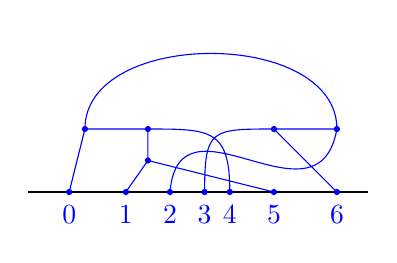
\begin{tikzpicture}[scale=0.8,even odd rule,baseline=0.5cm]
    \draw (6.1,0) -- (11.5,0);
    \draw[blue]
        (6.75,0) node[circle,fill,inner sep=0.8pt,label=below:$0$]{} -- (7,1) node[circle,fill,inner sep=0.8pt]{} -- (8,1) node[circle,fill,inner sep=0.8pt]{}
        -- (8,0.5) node[circle,fill,inner sep=0.8pt]{} -- (7.65,0) node[circle,fill,inner sep=0.8pt,label=below:$1$]{}
        (8,0.5)  -- (10,0) node[circle,fill,inner sep=0.8pt,label=below:$5$]{}
        (8,1) to[out=0,in=90,distance=1cm] (9.3,0)  node[circle,fill,inner sep=0.8pt,label=below:$4$]{}
        (8.9,0) node[circle,fill,inner sep=0.8pt,label=below:$3$]{} to[out=90,in=180,distance=1cm] (10,1) node[circle,fill,inner sep=0.8pt]{} -- (11,0) node[circle,fill,inner sep=0.8pt,label=below:$6$]{}
        (10,1) -- (11,1) node[circle,fill,inner sep=0.8pt]{} to[out=-100,in=85,distance=1.7cm] (8.35,0) node[circle,fill,inner sep=0.8pt,label=below:$2$]{}
        (11,1) to[out=90,in=90, distance=1.6cm]  (7,1) ;
\end{tikzpicture}
\\
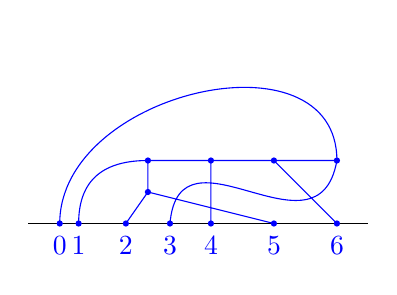
\begin{tikzpicture}[scale=0.8,even odd rule,baseline=0.5cm]
    \draw (6.1,0) -- (11.5,0);
    \draw[blue]
        (6.9,0) node[circle,fill,inner sep=0.8pt,label=below:$1$]{} to[out=90,in=180,distance=0.7cm] (8,1) node[circle,fill,inner sep=0.8pt]{} -- (8,0.5) node[circle,fill,inner sep=0.8pt]{} -- (7.65,0) node[circle,fill,inner sep=0.8pt,label=below:$2$]{}
        (8,0.5)  -- (10,0) node[circle,fill,inner sep=0.8pt,label=below:$5$]{}
        (8,1) -- (9,1) -- (9,0) node[circle,fill,inner sep=0.8pt,label=below:$4$]{}
        (9,1) node[circle,fill,inner sep=0.8pt]{} -- (10,1) node[circle,fill,inner sep=0.8pt]{} -- (11,0) node[circle,fill,inner sep=0.8pt,label=below:$6$]{}
        (10,1) -- (11,1) node[circle,fill,inner sep=0.8pt]{} to[out=-100,in=85,distance=1.7cm] (8.35,0) node[circle,fill,inner sep=0.8pt,label=below:$3$]{}
        (11,1) to[out=90,in=90, distance=2.1cm]  (6.6,0) node[circle,fill,inner sep=0.8pt,label=below:$0$]{} ;
\end{tikzpicture} 
&
$-$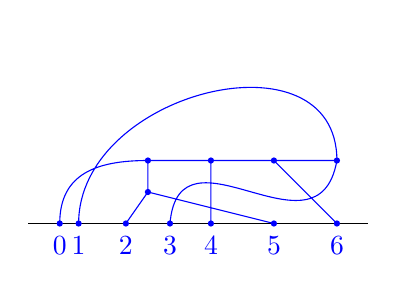
\begin{tikzpicture}[scale=0.8,even odd rule,baseline=0.5cm]
    \draw (6.1,0) -- (11.5,0);
    \draw[blue]
        (6.6,0) node[circle,fill,inner sep=0.8pt,label=below:$0$]{} to[out=90,in=180,distance=0.8cm] (8,1) node[circle,fill,inner sep=0.8pt]{} -- (8,0.5) node[circle,fill,inner sep=0.8pt]{} -- (7.65,0) node[circle,fill,inner sep=0.8pt,label=below:$2$]{}
        (8,0.5)  -- (10,0) node[circle,fill,inner sep=0.8pt,label=below:$5$]{}
        (8,1) -- (9,1) -- (9,0) node[circle,fill,inner sep=0.8pt,label=below:$4$]{}
        (9,1) node[circle,fill,inner sep=0.8pt]{} -- (10,1) node[circle,fill,inner sep=0.8pt]{} -- (11,0) node[circle,fill,inner sep=0.8pt,label=below:$6$]{}
        (10,1) -- (11,1) node[circle,fill,inner sep=0.8pt]{} to[out=-100,in=85,distance=1.7cm] (8.35,0) node[circle,fill,inner sep=0.8pt,label=below:$3$]{}
        (11,1) to[out=90,in=90, distance=2.1cm]  (6.9,0) node[circle,fill,inner sep=0.8pt,label=below:$1$]{} ;
\end{tikzpicture}
\end{tabular}
\end{document}